We propose the algorithm Latent Ranked Bandit, abbreviated as LRB (see Algorithm \ref{alg:latent-rank}) for solving the personalized ranking problem. This algorithm is motivated by the Ranked Bandit Algorithm (RBA) from \citet{radlinski2008learning} which is suited for finding a global ranking amongst all the users in the cascade based model. LRB is divided into two main components, the $d$ column MABs denoted by MAB$_1(n)$, MAB$_2(n), \dots,$ MAB$_d(n)$ and the $K$ row Weighted Majority Algorithms (WMA) for each user $[K]$. The WMA is motivated from \citet{littlestone1994weighted} which is suited for the total information setting. Note, that in our DCM setting all the clicks by the user is seen by the system and so it is also a specific variation of total information setting. Each WMA consist of $d$ arms for each of the ranks $1,2\dots,d$ and its main goal is to suggest the best item for the user in rank $1$.  LRB proceeds as follows, at every timestep as user $i_t$ is revealed by nature, the $d$ column MABs suggests columns ${\ell}_{1}, {\ell}_{2},\dots, {\ell}_{d}$ which it deems to be the $d$ best columns and by virtue of our setting, the $d$ hott-topics. If, there is any overlap in the suggestion, an arbitrary column is suggested which has not been selected before. Then, the row WMA for the $i_t$-th user selects a permutation $\Pi_{i_t}({\ell}_{1}, {\ell}_{2},\dots, {\ell}_{d})$ by sampling through its distribution over the $d$-ranks and suggests $\tilde{\ell}_{1}, \tilde{\ell}_{2},\dots, \tilde{\ell}_{d}$ such that the item in rank $1$ is the best item for the $i_t$-th user. 

Finally, after all the user clicks are recorded by the system both the column MABs and row WMA (for the $i_t$-th user only) is updated. The column bandits are updated with feedback $f_{k,t}$ such the monotonicity and submodularity properties discussed in section \ref{related} are maintained. Note that RBA is also a special case of submodular bandits such that $f_{k,t}\in\lbrace 0, 1\rbrace$ \citep{streeter2009online}. The row WMA update for the $i_t$-th user is quite straightforward as all the rewards for the $d$ clicks are observed. An illustrative diagram of the entire process is shown in Figure \ref{fig:rankedbandit}.


\begin{figure}[!th]
    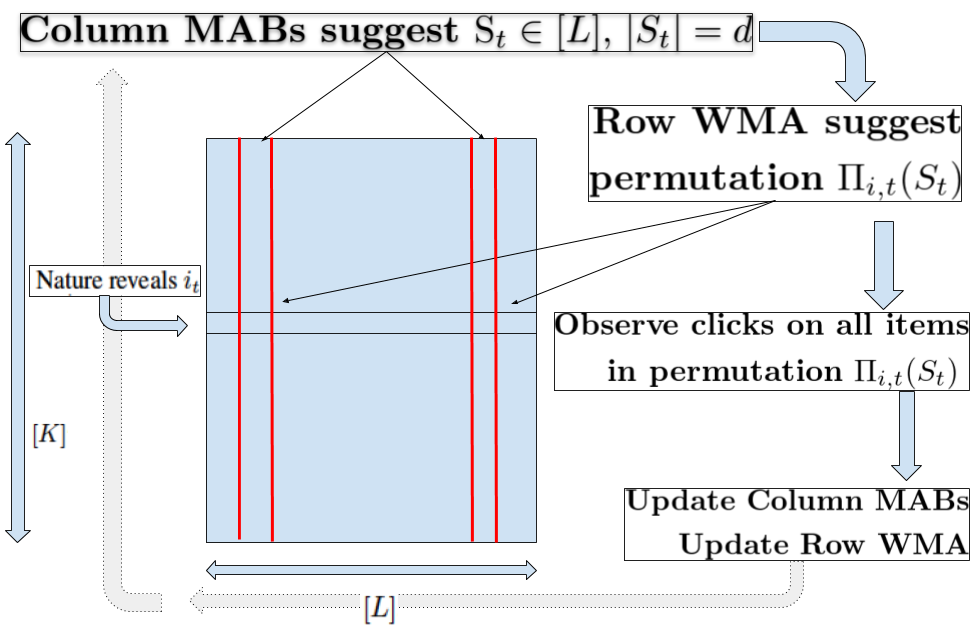
\includegraphics[scale=0.2]{img/RankedBand.png}
    \caption{Latent Ranked Bandit in rank $d=2$ scenario.}
    \label{fig:rankedbandit}
    \vspace*{-1em}
\end{figure}

\begin{algorithm}
\caption{Latent Ranked Bandit}
\label{alg:latent-rank}
  \begin{algorithmic}[1]
  \State \textbf{Input:} Rank $d$, horizon $n$.
  \State Initialize MAB$_1(n)$, MAB$_2(n), \dots,$ MAB$_d(n)$
  \State Initialize WMA$_1(n)$, WMA$_2(n), \dots,$ WMA$_K(n)$
    \For{$t = 1, \dots, n$}
      \State User $i_t$ comes to the system
      \For{$k = 1, \dots, d$}
      %\State // Choose $d$ items from $d$ column MABs
      \State ${\ell}_{k,t} \leftarrow$ suggest item $MAB_k(n)$
      \If{${\ell}_{k,t} \in \ell_{1, t},\dots,\ell_{k-1, t}$}
      \State ${\ell}_{k,t} \leftarrow$ Select arbitrary unselected item from $[L]\setminus \ell_{1, t},\dots,\ell_{k-1, t}$
      %\Else
      %\State $\ell_{k,t} \leftarrow \hat{\ell}_{k,t}$
      \EndIf
      \EndFor
      \State $\tilde{\ell}_{1,t},\tilde{\ell}_{2,t},\dots,\tilde{\ell}_{d,t}\leftarrow$ Permutation by WMA$_{i_t}(\ell_{1,t},\ell_{2,t},\dots,\ell_{d,t})$ by sorting descendingly according to $w_{i_t,1},w_{i_t,2},\dots,w_{i_t,d}$.
      \State Present $\tilde{\ell}_{1,t},\tilde{\ell}_{2,t},\dots,\tilde{\ell}_{d,t}$ to user $i_t$ and record feedback $r_{t}(\tilde{\ell}_{1,t}), r_{t}(\tilde{\ell}_{2,t}),\dots,r_{t}(\tilde{\ell}_{d,t})$.
      \State Call Procedure UpdateColumnMAB
      \State Call Procedure UpdateRowWMA($i_t$)
    \EndFor
    \Procedure{UpdateColumnMAB}{}
    \For{$k = 1, \dots, d$}
    \State Update MAB$_k(n)$ with feedback $f_{k,t} = \max_{j\in [k]} r_t(i_t, \ell_{j,t}) - \max_{j\in [k-1]} r_t(i_t,\ell_{j,t})$
    % where $J_t[1: k] = \lbrace r_{t}({\ell}_{1,t}), r_{t}({\ell}_{2,t}),\dots,r_{t}({\ell}_{k,t})\rbrace$
    \EndFor
\EndProcedure
\Procedure{UpdateRowWMA}{$i_t$}
    \For{$j = 1, \dots, d$}
    \State $w_{i_t,j} = w_{i_t,j} + \frac{1}{j}r_{t}(\tilde{\ell}_{j,t})$
    \EndFor
%    \For{$j = 1, \dots, d$}
%    \State $p_{i_t,j} = \dfrac{\exp(w_{i_t,j})}{\sum_{b=1}^d \exp(w_{i_t,b})} $
%    \EndFor
\EndProcedure
  \end{algorithmic}
\end{algorithm}